\documentclass[11pt]{article}
\usepackage[margin=1.1in]{geometry}
\usepackage{amsmath,amssymb,amsthm}
\usepackage[round]{natbib}
\usepackage{booktabs}
\usepackage{tikz}
\usepackage{hyperref}
\hypersetup{hidelinks}
\usepackage{microtype}

\newtheorem{theorem}{Theorem}
\newtheorem{proposition}[theorem]{Proposition}
\newtheorem{lemma}[theorem]{Lemma}
\newtheorem{corollary}[theorem]{Corollary}
\theoremstyle{definition}
\newtheorem{definition}[theorem]{Definition}
\newtheorem{assumption}{Assumption}
\theoremstyle{remark}
\newtheorem{remark}[theorem]{Remark}

\newcommand{\R}{\mathbb{R}}
\newcommand{\E}{\mathbb{E}}
\newcommand{\Prob}{\mathbb{P}}
\newcommand{\Var}{\mathrm{Var}}
\newcommand{\chis}{\chi^2}
\newcommand{\given}{\,|\,}

\title{What a Coverage Guarantee Costs:\\ the Price of Coverage at a Point}
\author{Peter Cotton}
\date{Working note, 27 September 2026}

\begin{document}
\maketitle

\begin{abstract}
Conformal prediction promises that its intervals cover the truth nine times in ten on
average over all inputs. A user usually wants that promise for the input in front of them.
We show what the stronger promise costs. Suppose similar inputs have similar error
distributions, and errors are spread out relative to their size. Then an interval that
covers nine times in ten at a given input, on average over the data used to build it, must
be wider than the interval someone who knew the true error distribution would quote. The
extra width is at least of order $n^{-s/(s+d)}$ in the number $n$ of past cases, which is
$n^{-1/2}$ with one input and the simplest smoothness assumption. For exponentially
distributed errors and that smoothness assumption we give a procedure that achieves it.
\end{abstract}

\section{The question}

\paragraph{What conformal prediction promises.}
Someone has a forecasting model and wants an interval around each forecast. Split conformal
prediction sets aside $n$ past cases, records how wrong the model was on each, and uses the
$90$th percentile of those errors as the half-width of every interval. The promise is that
the interval contains the truth $90\%$ of the time. The probability in that promise is an
average over everything random, including which input turns up next. It is called
\emph{marginal} coverage.

\paragraph{What people want.}
A user with a particular input in hand wants to know about that input. A patient is not
reassured by a rate that averages over all patients. Marginal coverage permits $99\%$
coverage on easy inputs and $60\%$ on hard ones, provided they average to $90\%$. So the
natural request is coverage \emph{at the input}.

\paragraph{What is known.}
With no assumption at all, coverage at every input is impossible with intervals of finite
width \citep{vovk2012conditional,lei2014distribution,barber2021limits}. With an assumption
that the error distribution changes smoothly with the input, it becomes possible: nearby
past cases are informative about this one. But it cannot be free. The interval must be
wider than the ideal one that a person who knew the true error distribution would quote.

\paragraph{The question.}
How much wider? The answer depends on what, exactly, is promised at the input. The past
cases are themselves a random draw, and there are two ways to treat that.
\begin{itemize}
\item \emph{In expectation.} The interval at this input covers $90\%$ of the time, counting
  both the luck of the next outcome and the luck of which past cases were drawn. This is what
  a textbook prediction interval promises.
\item \emph{With high probability.} On most possible draws of the past cases, say nine in ten,
  the interval built from that draw covers at least $90\%$ of the time at this input.
  Nothing is averaged away: a bad draw of past cases counts as a failure.
\end{itemize}
Neither promise implies the other. The first allows an occasional draw on which coverage at
this input is poor, provided the average is right. The second allows one draw in ten on
which coverage is anything at all, even zero, so its average coverage can be as low as
$81\%$. What the second promise forces is worked out in \citet{cotton2026honest}, using
the theory of confidence intervals of \citet{low1997nonparametric} and
\citet{cai2004adaptation}. We have not found what the first forces in print. This note computes it.

\paragraph{The result.}
Three numbers govern the answer. The number of past cases is $n$. The number of input
variables is $d$. The smoothness $s$ says how regularly the error distribution changes with
the input: $s=1$ means it changes at a bounded rate, and larger $s$ means smoother. All
three are defined precisely in Section~\ref{sec:setup}.

Table~\ref{tab:prices} lists each promise with what it forces. An entry such as $n^{-1/2}$
means a quantity proportional to $1/\sqrt n$, so a hundred times more data makes it ten
times smaller. The second row is the contribution of this note.

The rows are not measured in the same way, and the difference matters. For the promise in
expectation we bound the \emph{average} threshold over draws. For the promise on most draws
the known result bounds the threshold on a \emph{typical} draw: on more than half of draws
it exceeds the ideal by the stated amount. The average would be the wrong measure there,
because that promise lets a procedure quote zero on a few draws, which lowers its average
threshold without breaking the promise.

\begin{table}[h]
\centering\small\setlength{\tabcolsep}{4pt}
\begin{tabular}{llll}
\toprule
Promise at the input & Forced above the ideal & $s=d=1$ & Source \\
\midrule
None (averaged over inputs) & nothing & & \citet{lei2014distribution} \\
Averaged over draws & average threshold, by $n^{-s/(s+d)}$ & $n^{-1/2}$ &
  this note \\
On most draws & typical threshold, by $n^{-s/(2s+d)}$ & $n^{-1/3}$ &
  \citet{cotton2026honest} \\
On every draw & threshold, by a fixed amount$^{*}$ & & \citet{cotton2026honest} \\
With no smoothness assumed & infinite width & & \citet{barber2021limits} \\
\bottomrule
\end{tabular}
\caption{What each promise forces. The first row says the marginal promise forces nothing: a
procedure can keep it and still approach the ideal interval as fast as the ideal interval
can be estimated. The second and third promises are not ordered, neither implies the other,
and their costs are measured differently. The fourth implies both. $^{*}$When the error
size is known to lie in a bounded range. With no such bound the fourth promise forces an
infinite threshold.}
\label{tab:prices}
\end{table}

\paragraph{An example with numbers.}
The example is fully specified as follows.
\begin{itemize}
\item \emph{Inputs.} One input variable, taking values between $0$ and $1$. The $n$ past
  cases have evenly spaced inputs $x_i=(i-\tfrac12)/n$, and the input we care about is
  $x_0=\tfrac12$. Even spacing is used so that the numbers are exact. The theorems treat
  inputs placed at random.
\item \emph{Scores.} The \emph{score} of a past case is the size of the model's error on
  it. Given the input $x$, the score is exponentially distributed with mean $e^{\theta(x)}$,
  where $\theta$ is a function of the input that the procedure does not know. This is a choice made so that every number below is exact and not
  simulated. It is the distribution of the absolute error when errors follow a Laplace
  distribution. Writing the mean as $e^{\theta}$ keeps it positive and puts $\theta$ on a
  log scale, so that a change of $0.1$ in $\theta$ means errors about $10\%$ larger.
\item \emph{The truth.} $\theta(x)=0$ for every $x$. So every score, at every input, is
  exponential with mean one. The procedure is not told this.
\item \emph{What the procedure is told.} That $\theta$ changes by at most $1$ per unit
  distance. In the notation of Section~\ref{sec:setup} this is smoothness $s=1$ with
  constant $L=1$. The procedure must keep its promise for every such $\theta$, not only the
  true one.
\item \emph{Target.} $90\%$ coverage at $x_0$, so $\alpha=0.1$.
\end{itemize}
The \emph{oracle threshold} is the $90$th percentile of an exponential with mean one, which
is $\log 10=2.303$. Someone who knew the truth would quote exactly that, and nothing smaller
covers $90\%$ of the time.

A \emph{threshold} is the number a procedure quotes as the largest error it expects at
$x_0$, so the interval is the forecast plus or minus the threshold. A procedure that does
not know the truth quotes a threshold that depends on the data, so we report its average
over draws of the scores. Both procedures below multiply the average
score of the $k$ nearest past cases by a constant, as in Section~\ref{sec:attain}, with $k$
chosen to make the average threshold as small as possible.

\begin{center}\setlength{\tabcolsep}{5pt}
\begin{tabular}{lrrrr}
\toprule
 & \multicolumn{2}{c}{$n=10{,}000$} & \multicolumn{2}{c}{$n=1{,}000{,}000$} \\
Promise at $x_0$ & average threshold & above oracle & average threshold & above oracle \\
\midrule
Oracle, knows the truth & $2.303$ & & $2.303$ & \\
In expectation & $2.338$ & $1.5\%$ & $2.306$ & $0.15\%$ \\
On $90\%$ of draws & $2.502$ & $8.7\%$ & $2.344$ & $1.8\%$ \\
\bottomrule
\end{tabular}
\end{center}

\noindent The in-expectation procedure uses $k=148$ neighbours at $n=10{,}000$ and the
other uses $k=564$. With a hundred times more data the first excess falls by a factor of
ten, which is $100^{1/2}$. The second falls by a factor of $4.8$, close to
$100^{1/3}=4.6$. The theorems below show that no procedure keeping the first promise can
improve on the ``in expectation'' row by more than a constant factor.

The last row needs a caution. It is the average threshold of one procedure that keeps the
second promise by padding on every draw. A procedure may instead quote zero on $8\%$ of
draws and pad the rest a little more. It still keeps the second promise, and at
$n=1{,}000{,}000$ its average threshold is $2.170$, below the oracle. So the last row is
what a sensible procedure costs, not what the promise forces on the average. No coin is
needed for this. A procedure can quote zero whenever the first past case has an input below
$0.08$, which happens on $8\%$ of draws when inputs are placed at random and tells it
nothing about $x_0$.

\paragraph{Why the two prices differ.}
Any threshold computed from data wobbles from one draw of the data to the next. Suppose it
wobbles evenly above and below the ideal value. Under the in-expectation promise the draws
that land too high nearly cancel the draws that land too low. They do not cancel exactly,
because landing too low loses more coverage than landing equally too high gains. What is left
over is proportional to the \emph{square} of the wobble.

The reason is that coverage is a curved function of the threshold. Raising the threshold
from $t$ to $t+w$ adds the probability that the score lands between them, and scores are
scarcer the further out one goes, so each further step adds less than the one before. In
the example above the oracle threshold $2.303$ covers $90\%$. A threshold $0.5$ higher
covers $93.9\%$, a gain of $3.9$ points. A threshold $0.5$ lower covers $83.5\%$, a loss of
$6.5$ points. A procedure that quotes each half the time is right on average about the
threshold and covers $88.7\%$, short by $1.3$ points. Halve the wobble to $0.25$ and the
shortfall is $0.31$ points, a quarter of what it was. A straight line would give no
shortfall at all, and the first departure of a smooth curve from its tangent line is
quadratic. To restore $90\%$ the procedure must raise its thresholds by an amount
proportional to the shortfall, hence to the square of the wobble.
Figure~\ref{fig:curve} shows the three thresholds.

\begin{figure}[h]
\centering
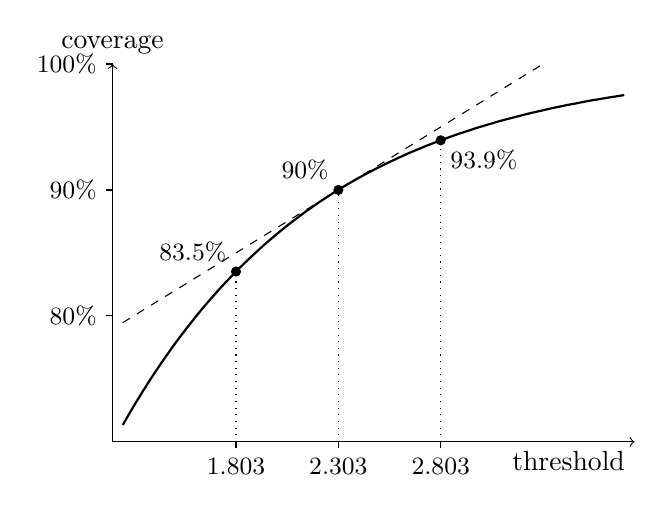
\begin{tikzpicture}[xscale=2.6,yscale=16]
  \draw[->] (1.2,0.70) -- (3.75,0.70) node[below left] {threshold};
  \draw[->] (1.2,0.70) -- (1.2,1.0) node[above] {coverage};
  \foreach \y/\l in {0.8/80\%,0.9/90\%,1.0/100\%} \draw (1.2,\y) -- (1.17,\y) node[left] {\small \l};
  \foreach \x in {1.803,2.303,2.803} \draw (\x,0.70) -- (\x,0.695) node[below] {\small \x};
  \draw[thick,domain=1.25:3.7,samples=80] plot (\x,{1-exp(-\x)});
  \draw[dashed,domain=1.25:3.3] plot (\x,{0.9+0.1*(\x-2.303)});
  \draw[dotted] (1.803,0.70) -- (1.803,0.8352);
  \draw[dotted] (2.303,0.70) -- (2.303,0.9);
  \draw[dotted] (2.803,0.70) -- (2.803,0.9394);
  \node[circle,fill,inner sep=1.3pt] at (1.803,0.8352) {}; \node[above left] at (1.803,0.8352) {\small $83.5\%$};
  \node[circle,fill,inner sep=1.3pt] at (2.303,0.9) {}; \node[above left] at (2.303,0.9) {\small $90\%$};
  \node[circle,fill,inner sep=1.3pt] at (2.803,0.9394) {}; \node[below right] at (2.803,0.9394) {\small $93.9\%$};
\end{tikzpicture}
\caption{Coverage as a function of the threshold, for scores that are exponential with mean
one. The solid curve bends downward. The dashed line is the straight line touching it at the
oracle threshold $2.303$. Moving $0.5$ below the oracle loses $6.5$ points of coverage, and
moving $0.5$ above gains $3.9$.}
\label{fig:curve}
\end{figure}

Under the high-probability promise nothing cancels. On each of the draws that count, the
threshold must itself be high enough, so it is padded by the wobble and not by its square. A
squared small number is much smaller, so the in-expectation promise can tolerate more
wobble. It therefore borrows from fewer, closer past cases, which reduces the error from
treating neighbours as identical.

\paragraph{Why this matters for conformal prediction.}
It separates two statements that are often run together. Conformal prediction's own
guarantee is nearly free and says nothing about any particular input. Every guarantee that
does say something about a particular input has a price, the price can be written down, and
it is paid in width.

\paragraph{How the note is organized.}
Section~\ref{sec:setup} defines every term. Section~\ref{sec:results} states the two
results in words. Section~\ref{sec:assump} states the assumptions and says when each fails.
Section~\ref{sec:lower} proves that no procedure can do better than the stated rate.
Section~\ref{sec:exp} checks the assumptions in the model of the example and gives
numerical constants. Section~\ref{sec:attain} gives a procedure that achieves the rate.
Section~\ref{sec:reading} says what the result means, what it does not show, and what is
borrowed from earlier work. A reader who wants the idea and not the proofs can stop after
Section~\ref{sec:results} and resume at Section~\ref{sec:reading}.

\section{Setup and definitions}\label{sec:setup}

\paragraph{Inputs, outcomes, scores.}
An \emph{input} is a vector $x\in\R^d$. A forecasting model has already been fitted on other
data and is not changed again, and we call it \emph{frozen}. For an input $X$ with outcome
$Y$, the \emph{score} $R\ge0$ measures how wrong the frozen model was, for example
$R=|Y-\hat\mu(X)|$ where $\hat\mu$ is the model's forecast. Large scores are large errors.

\paragraph{Calibration sample.}
The \emph{calibration sample} $D_n=\{(X_i,R_i)\}_{i=1}^n$ is a set of $n$ past cases, not
used to fit the model. The pairs are independent draws from one distribution. The inputs
$X_i$ have probability density $g$ on $\R^d$. The positions of the inputs $X_1,\dots,X_n$
are called the \emph{design}.

\paragraph{How the score distribution depends on the input.}
We describe the distribution of the score at input $x$ by one number $\theta(x)$, such as
the log of the typical error size there. Formally there is a family of distribution
functions $\{F_u\}$ indexed by a real number $u$, and
\[
  \Prob(R\le t\given X=x)\;=\;F_{\theta(x)}(t).
\]
The function $\theta:\R^d\to\R$ is unknown. We call it the \emph{field}. A single parameter
is enough for a lower bound: if the true family has more parameters, a lower bound proved
for a one-parameter slice of it still holds.

\paragraph{Test point.}
The \emph{test point} $x_0$ is a fixed input chosen in advance. It is not random.

\paragraph{Procedure, threshold, prediction set.}
A \emph{procedure} is a rule that turns the calibration sample into a number $T\ge0$, the
\emph{threshold}. The \emph{prediction set} for the score at $x_0$ is $[0,T]$: the
procedure asserts that the model's error at $x_0$ will be at most $T$. For the absolute
error score this is the interval $\hat\mu(x_0)\pm T$. The rule may also flip coins. We write
$T=T(D_n,U)$ with $U$ the coin flips, independent of the data.

\paragraph{Miscoverage level and oracle threshold.}
Fix $\alpha\in(0,1)$, the permitted failure rate, so that $1-\alpha$ is the target
coverage. With $\alpha=0.1$ the target is $90\%$. The \emph{oracle threshold} is the
threshold someone who knew the true distribution at $x_0$ would quote,
\[
  q_\alpha(u)\;=\;F_u^{-1}(1-\alpha)\qquad\text{at }u=\theta(x_0),
\]
the $(1-\alpha)$ quantile of the score at $x_0$. No threshold below it achieves the target.

\paragraph{The guarantee.}
Write $\E_\theta$ and $\Prob_\theta$ for expectation and probability over the calibration
sample and the coin flips when the field is $\theta$. For a realized threshold $T$, the
chance that a fresh score at $x_0$ falls below it is $F_{\theta(x_0)}(T)$. This is the
coverage achieved by that particular $T$, and it is random because $T$ is.

\begin{definition}[Validity at a point in expectation]\label{def:valid}
Let $\Theta$ be a set of fields. A procedure is \emph{valid at $x_0$ in expectation over
$\Theta$} if
\begin{equation}\label{eq:valid}
  \E_\theta\big[F_{\theta(x_0)}(T)\big]\;\ge\;1-\alpha
  \qquad\text{for every }\theta\in\Theta .
\end{equation}
\end{definition}

Equivalently $\Prob_\theta(R_0\le T)\ge1-\alpha$ where $R_0$ is a fresh score at $x_0$,
independent of the calibration sample and the coin flips, and
the probability runs over both $R_0$ and the calibration sample. The requirement must hold
for every field in $\Theta$, because the procedure does not know which one is true.

For comparison, \emph{marginal} validity replaces the fixed $x_0$ by a random input $X_0$
drawn from $g$ and averages over it as well. \emph{High-probability} validity at level
$1-\eta$ asks that $\Prob_\theta\{F_{\theta(x_0)}(T)\ge1-\alpha\}\ge1-\eta$. Validity at
$x_0$ for every $x_0$ implies marginal validity. High-probability validity with $\eta>0$
does not imply validity in expectation: it guarantees only
$\E_\theta F_{\theta(x_0)}(T)\ge(1-\eta)(1-\alpha)$. Nor does validity in expectation imply
high-probability validity.

\paragraph{The cost.}
The \emph{excess} of a procedure under the field $\theta$ is how far its threshold sits
above the oracle's on average,
\[
  \Delta_\theta(T)\;=\;\E_\theta[T]-q_\alpha\big(\theta(x_0)\big),
\]
with $\Delta_\theta=\infty$ if $\E_\theta T=\infty$. For an interval $\hat\mu(x_0)\pm T$ it
is half the expected extra width. We ask how small the excess can be made for a valid
procedure. Since the procedure does not know the field, we look at its excess in the worst
case over the fields it must allow for, written $\sup_{\theta\in\Theta}\Delta_\theta(T)$.

\paragraph{Smoothness.}
The assumption that makes the problem possible is that the field does not change abruptly.
For $0<s\le1$ and $L>0$, the field $\theta$ is \emph{H\"older smooth of order $s$ with
constant $L$} if
\[
  |\theta(x)-\theta(y)|\;\le\;L\,|x-y|^{s}\qquad\text{for all }x,y .
\]
With $s=1$ this says $\theta$ changes by at most $L$ per unit distance. For $s>1$, write
$k$ for the largest integer strictly below $s$. The condition is that $\theta$ has
derivatives up to order $k$ and that every derivative of order $k$ satisfies the display
above with exponent $s-k$. We write $\mathcal H^s(L)$ for the set of such fields and call it
the \emph{H\"older ball}. Larger $s$ means smoother, and larger $L$ means rougher.

\paragraph{Bandwidth.}
Any procedure that uses past cases near $x_0$ must decide how near. The radius $h$ of the
neighbourhood it uses is the \emph{bandwidth}. A neighbourhood of radius $h$ holds about
$n\,g(x_0)\,h^d$ past cases, up to a constant. A wide neighbourhood holds many cases, so
averages over it are steady, but those cases are less like $x_0$. The error from treating
neighbours as if they sat at $x_0$ is the \emph{bias}. For $s\le1$ it is at most $Lh^s$.
For $s>1$ the field may have a slope, so a plain average of neighbours can be off by more,
and a bias of order $Lh^s$ is reached only after fitting and removing the slope and the
higher terms up to order $k$.

\paragraph{A distance between distributions.}
For two probability distributions $P$ and $Q$, with $P$ having density $dP/dQ$ relative to
$Q$, the \emph{chi-square divergence} is
\[
  \chis(P\,\|\,Q)\;=\;\int\Big(\frac{dP}{dQ}\Big)^{2}dQ-1 .
\]
It is zero when $P=Q$ and grows as they separate. It measures how hard it is to tell from
data which of the two produced it. It is not symmetric in $P$ and $Q$.

\section{Results}\label{sec:results}

The first result says validity is expensive in a specific way.

\begin{theorem}[Lower bound, informal]
Suppose past cases are neither absent nor piled up near $x_0$
(Assumption~\ref{as:design}), and the scores are spread out relative to their size, as
exponential or half-normal scores are (Assumption~\ref{as:family}). Let $\theta_0$ be a
constant field, so that the score distribution is the same at every input. Then for all large $n$, every procedure valid
at $x_0$ in expectation over $\mathcal H^s(L)$ has
\[
  \Delta_{\theta_0}(T)\;\ge\;
  c\;L^{d/(s+d)}\,\big(n\,g_+\big)^{-s/(s+d)},
\]
where $g_+$ is an upper bound on the density of inputs near $x_0$, so that $n\,g_+$ measures
how many past cases fall near $x_0$, and $c>0$ does not depend on $n$ or $L$.
\end{theorem}

The excess is forced when the truth is the simplest field in the class, the one with no
variation at all. The procedure pays for bumps that are not there, because it cannot rule
them out.

The precise version is Corollary~\ref{cor:rate}. The second result says the bound cannot be
improved.

\begin{theorem}[Attainment, informal]
When scores are exponentially distributed with a mean that varies smoothly with the input,
the log of that mean is known to lie in a bounded range, and $s\le1$, there is an explicit
procedure that is valid at $x_0$ in expectation for every
$n$, with no approximation, and whose excess is at most
$C\,L^{d/(s+d)}(n\,g_-)^{-s/(s+d)}$ under every field in the class. Here $g_-$ is a lower
bound on the density of inputs near $x_0$ and $C$ does not depend on $n$ or $L$.
\end{theorem}

The precise version is Proposition~\ref{prop:upper}. The two bounds have the same
dependence on $n$ and on $L$ and differ only in their constants. Together they give the
second row of Table~\ref{tab:prices}.

The factor $L^{d/(s+d)}$ says that a rougher class costs more. If $L=0$ the field is known
to be constant, every past case is as good as a case at $x_0$, and the bound vanishes.

\section{Assumptions}\label{sec:assump}

\begin{assumption}[The input density is bounded near the test point]\label{as:design}
There are a radius $r_0>0$ and constants $0<g_-\le g_+<\infty$ with $g_-\le g(x)\le g_+$
for all $x$ within distance $r_0$ of $x_0$.
\end{assumption}

This says past cases near $x_0$ are neither absent nor piled up. It fails at the edge of
the data and in sparse regions.

\begin{assumption}[The score family is regular near a baseline]\label{as:family}
There are a baseline value $u_0$, a width $\varepsilon_0>0$ and positive constants
$K,c_q,C_q,\bar f,\kappa,\rho$ such that for all $u\in[u_0,u_0+\varepsilon_0]$:
\begin{enumerate}
\item[(a)] \emph{Nearby parameters are hard to tell apart.}
  $\chis(F_u\,\|\,F_{u_0})\le K(u-u_0)^2$.
\item[(b)] \emph{The oracle threshold moves with the parameter.}
  $c_q(u-u_0)\le q_\alpha(u)-q_\alpha(u_0)\le C_q(u-u_0)$.
\item[(c)] \emph{The distribution function bends downward at the oracle threshold.} $F_u$
  has a density, its value at the oracle threshold $f_u:=F_u'(q_\alpha(u))$ satisfies
  $0<f_u\le\bar f$, and for every $t\ge0$
  \begin{equation}\label{eq:gap}
    F_u(t)\;\le\;1-\alpha+f_u\,\big(t-q_\alpha(u)\big)-\kappa\,\psi_\rho\big(t-q_\alpha(u)\big),
    \qquad \psi_\rho(v):=\min\{v^2,\rho|v|\}.
  \end{equation}
\end{enumerate}
\end{assumption}

The constants have these roles. $K$ says how fast two score distributions become
distinguishable as their parameters separate. The divergence is proportional to the
\emph{square} of the separation because that is how every smooth family behaves for small
separations. $c_q$ and $C_q$ say how fast the oracle threshold moves when the parameter
moves. $\bar f$ bounds the score density at the oracle threshold. $\kappa$ and $\rho$
describe the curvature of the distribution function and are explained next.

Part (c) carries the argument. The first two terms on the right
of \eqref{eq:gap} are the straight line touching the graph of $F_u$ at the oracle threshold.
The inequality says the graph lies below that line, by an amount that is quadratic in the
distance $v$ from the threshold when $v$ is small and linear when $v$ is large. The function
$\psi_\rho$ is that amount, and $\rho$ is where it changes from quadratic to linear. It is
the mathematical form of ``landing too low loses more than landing too high gains''.

The condition is required for every $t\ge0$, including $t=0$, and that makes it a
restriction on the family. At $t=0$ the left side is zero, and with $q=q_\alpha(u)$ the
condition reads $q\,f_u\le1-\alpha-\kappa\,\psi_\rho(q)$. In particular it needs
$q\,f_u<1-\alpha$. This holds for scores that are spread out relative to their size and
fails for scores concentrated near a positive value. With $\alpha=0.1$ the product $q\,f_u$
is $0.23$ for the exponential, $0.34$ for the absolute value of a normal, and $0.86$ for a
gamma distribution with shape $20$, all of which qualify. It is $1.03$ for a gamma with
shape $30$ and $1.15$ for a Weibull with shape $5$, which do not. A decreasing density at the
threshold is not enough.

The restriction is not an artefact of the proof. For the gamma with shape $30$ the oracle
threshold is $37.199$, and a procedure that quotes $0$ with small probability and $37.80$
otherwise covers $90\%$ of the time with an average threshold of $37.155$. That is below
the oracle. So for concentrated scores the excess as we have defined it can be negative,
and a different measure of cost is needed.

\begin{assumption}[The class contains a small local bump]\label{as:holder}
The set of fields is $\Theta=\mathcal H^s(L)$. There is a function $b:\R^d\to[0,1]$, the
\emph{bump profile}, with $b(0)=1$ and $b(z)=0$ for $|z|\ge1$, and there are constants
$a\in(0,1]$ and $h_0\in(0,r_0]$, such that for every $0<h\le h_0$ the two fields
\[
  \theta_0(x)=u_0
  \qquad\text{and}\qquad
  \theta_1(x)=u_0+a\,L\,h^{s}\,b\Big(\frac{x-x_0}{h}\Big)
\]
both belong to $\Theta$. Write $\|b\|_2^2=\int b(z)^2dz$.
\end{assumption}

The field $\theta_0$ is flat. The field $\theta_1$ equals $\theta_0$ except within distance
$h$ of $x_0$, where it rises to a peak of height $aLh^s$ at $x_0$. A bump of width $h$ can
be at most about $Lh^s$ tall and still be H\"older smooth, which is why the height has that
form. The constant $a$ is whatever is needed to keep the bump inside the ball. For $s=d=1$
the triangle $b(z)=\max\{1-|z|,0\}$ works with $a=1$. Figure~\ref{fig:bump} shows the two
fields.

\begin{figure}[h]
\centering
\begin{tikzpicture}[xscale=1.6,yscale=1.4]
  \draw[->] (0,0) -- (6.3,0) node[below] {input $x$};
  \draw[->] (0,0) -- (0,2.1) node[above] {$\theta(x)$};
  \draw[thick] (0.2,0.8) -- (6,0.8) node[right] {$\theta_0$};
  \draw[thick,dashed] (0.2,0.8) -- (2.2,0.8) -- (3.1,1.7) -- (4.0,0.8) -- (6,0.8);
  \node[above] at (3.1,1.7) {$\theta_1$};
  \draw[dotted] (3.1,0) -- (3.1,1.7);
  \node[below] at (3.1,0) {$x_0$};
  \draw[<->] (2.2,0.35) -- (3.1,0.35) node[midway,below] {\small $h$};
  \draw[<->] (4.25,0.8) -- (4.25,1.7) node[midway,right] {\small $aLh^{s}$};
  \draw (0,0.8) -- (-0.06,0.8) node[left] {$u_0$};
  \foreach \x in {0.35,0.8,1.3,1.75,2.4,2.75,3.0,3.35,3.8,4.4,4.9,5.3,5.8} \node[circle,fill,inner sep=1pt] at (\x,0) {};
\end{tikzpicture}
\caption{The flat field $\theta_0$ (solid) and the bump field $\theta_1$ (dashed). Dots are
the inputs of past cases. Only the few cases under the bump carry any information about
which field is true. A narrower bump is lower and covers fewer cases, so it is harder to
detect.}
\label{fig:bump}
\end{figure}

\section{The lower bound}\label{sec:lower}

\paragraph{Plan.}
The two fields $\theta_0$ and $\theta_1$ differ only near $x_0$, so a calibration sample
drawn under one looks much like a sample drawn under the other. A valid procedure must cover
under both. Under $\theta_1$ the oracle threshold is higher, so the procedure's threshold
must be higher on average. It cannot meet that requirement with rare enormous thresholds,
because coverage cannot exceed one: beyond a certain size a larger threshold buys nothing.
And a procedure cannot behave very differently on samples it cannot tell apart, unless its
threshold varies a great deal. Lemma~\ref{lem:curv} shows validity itself limits how much
the threshold may vary. Together these force the excess up under the flat field.

\begin{lemma}[Validity bounds the spread by the excess]\label{lem:curv}
Let Assumption~\ref{as:family}(c) hold at $u=\theta(x_0)$, write $q=q_\alpha(u)$, and let
$T$ satisfy \eqref{eq:valid} under $\theta$ with $\E_\theta T<\infty$. Then
\[
  \Delta_\theta\ge 0
  \qquad\text{and}\qquad
  \E_\theta\,\psi_\rho(T-q)\;\le\;\frac{\bar f}{\kappa}\,\Delta_\theta .
\]
\end{lemma}

In words: a valid threshold sits above the oracle on average, and its typical squared
distance from the oracle is at most a constant times its excess.

\begin{proof}
Put $t=T$ in \eqref{eq:gap} and take expectations. The left side is at least $1-\alpha$ by
\eqref{eq:valid}, and $\E_\theta(T-q)=\Delta_\theta$, so
$1-\alpha\le 1-\alpha+f_u\Delta_\theta-\kappa\,\E_\theta\psi_\rho(T-q)$. That is
$\kappa\,\E_\theta\psi_\rho(T-q)\le f_u\Delta_\theta$. The left side is nonnegative and
$f_u>0$, so $\Delta_\theta\ge0$. Then $f_u\Delta_\theta\le\bar f\Delta_\theta$ gives the
second claim.
\end{proof}

\begin{lemma}[Change of expectation]\label{lem:chi}
Let $P_0$ and $P_1$ be probability distributions with $P_1$ having a density relative to
$P_0$, and let $Y$ be a random variable with finite variance under $P_0$. Writing $\E_j$
and $\Var_j$ for expectation and variance under $P_j$,
\[
  \big(\E_1Y-\E_0Y\big)^2\;\le\;\chis(P_1\|P_0)\,\Var_0(Y).
\]
\end{lemma}

In words: if two distributions are hard to tell apart, the average of any quantity can
differ between them only if that quantity is highly variable.

\begin{proof}
With $\Lambda=dP_1/dP_0$ we have $\E_0\Lambda=1$, so
$\E_1Y-\E_0Y=\E_0[(\Lambda-1)(Y-\E_0Y)]$. The Cauchy--Schwarz inequality bounds the square
of this by $\E_0(\Lambda-1)^2\cdot\Var_0(Y)$, and $\E_0(\Lambda-1)^2=\chis(P_1\|P_0)$. This
is Lemma~2.1 of \citet{derumigny2023lower}.
\end{proof}

\begin{theorem}[Two-point bound at the flat field]\label{thm:two}
Let Assumptions~\ref{as:design}--\ref{as:holder} hold. Fix a bump width $h\in(0,h_0]$, let
$\delta=aLh^s$ be the bump height, and suppose
\begin{equation}\label{eq:cond}
  \delta\le\varepsilon_0,\qquad
  C_q\,\delta\le\rho/2,\qquad
  I:=n\,K\,g_+\,\|b\|_2^2\,\delta^2h^d\le 1 .
\end{equation}
Then every procedure satisfying \eqref{eq:valid} under both $\theta_0$ and $\theta_1$ has
\begin{equation}\label{eq:two}
  \Delta_{\theta_0}(T)
  \;\ge\;
  \min\Big\{\,A_1\,L\,h^{s},\;\frac{A_2}{n\,g_+\,h^{d}}\Big\},
\end{equation}
with, writing $q_0=q_\alpha(u_0)$,
\[
  A_1=\frac{c_q\,a}{2},\qquad
  A_2=\frac{\kappa\,c_q^2}{8\,\bar f\,C_{\mathrm{cap}}\,K\,\|b\|_2^2},\qquad
  C_{\mathrm{cap}}=\max\Big\{1,\;\frac{q_0}{\rho},\;\frac12+\frac{\alpha}{\kappa\rho^2}\Big\}.
\]
\end{theorem}

The constants $A_1$, $A_2$ and $C_{\mathrm{cap}}$ depend on the score family, the target
$\alpha$ and the bump profile. They do not depend on $n$, $L$ or $h$.

The three conditions in \eqref{eq:cond} say the bump is small enough for
Assumption~\ref{as:family} to apply, small enough that the two oracle thresholds are close,
and small enough that the two fields are hard to tell apart from $n$ observations. The
quantity $I$ measures the last: it is the bump height squared times the number of past
cases under the bump. The two terms on the right of \eqref{eq:two} are the bias a bandwidth
$h$ can hide, and the reciprocal of the number of past cases within $h$ of $x_0$.

\begin{proof}
Write $P_j$ for the distribution of the sample and coin flips $(D_n,U)$ under $\theta_j$,
and $\E_j$ for expectation under it. Write $q_1=q_\alpha(u_0+\delta)$ for the oracle
threshold under the bump field, $\gamma=q_1-q_0$, $F_1=F_{u_0+\delta}$ and
$f_1=f_{u_0+\delta}$. Since $b(0)=1$ we have $\theta_1(x_0)=u_0+\delta$, and
Assumption~\ref{as:family}(b) gives $c_q\delta\le\gamma\le C_q\delta\le\rho/2$. Write
$\Delta_0=\Delta_{\theta_0}$. If $\Delta_0=\infty$ there is nothing to prove, so assume
$\E_0T<\infty$. Let $v=T-q_0$.

\emph{Step 1: cap the threshold where coverage saturates.} Dropping the last term of
\eqref{eq:gap} gives $F_1(T)\le1-\alpha+f_1(T-q_1)=1-\alpha+f_1(v-\gamma)$. Also
$F_1(T)\le1$. Put
\[
  B=\gamma+\frac{\alpha}{f_1},\qquad Z=\min\{v,B\}.
\]
Then, for every value of $T$,
\[
  F_1(T)\;\le\;\min\big\{1,\;1-\alpha+f_1(v-\gamma)\big\}\;=\;1-\alpha+f_1(Z-\gamma).
\]
Taking expectations under the bump field and using \eqref{eq:valid},
$1-\alpha\le1-\alpha+f_1(\E_1Z-\gamma)$, so
\begin{equation}\label{eq:e1}
  \E_1Z\;\ge\;\gamma .
\end{equation}
The variable $Z$ is bounded, since $-q_0\le Z\le B$, so no assumption on $\E_1T$ is needed.

\emph{Step 2: the density at the threshold exceeds $\kappa\rho$.} For $t>q_1+\rho$ the
right side of \eqref{eq:gap} is $1-\alpha+(f_1-\kappa\rho)(t-q_1)$. The left side tends to
$1>1-\alpha$ as $t\to\infty$. So $f_1>\kappa\rho$, and with $\gamma\le\rho/2$,
\[
  \frac{B}{\rho}\;\le\;\frac12+\frac{\alpha}{\kappa\rho^2}\;\le\;C_{\mathrm{cap}}.
\]

\emph{Step 3: under the flat field, $Z$ has small mean and small variance.} Since
$Z\le v$,
\begin{equation}\label{eq:e0}
  \E_0Z\;\le\;\E_0v\;=\;\Delta_0 .
\end{equation}
We claim $Z^2\le C_{\mathrm{cap}}\,\psi_\rho(v)$. Note $B>0$. If $|v|\le\rho$, then
$|Z|\le|v|$ and $Z^2\le v^2=\psi_\rho(v)$. If $v<-\rho$, then $Z=v$ and $|v|\le q_0$
because $T\ge0$, so $Z^2=|v|^2\le q_0|v|=(q_0/\rho)\,\psi_\rho(v)$. If $v>\rho$, then
$0<Z\le B$ and $Z\le v$, so $Z^2\le Bv=(B/\rho)\,\psi_\rho(v)$. In each case the constant
is at most $C_{\mathrm{cap}}$. Lemma~\ref{lem:curv} under $\theta_0$ now gives
\begin{equation}\label{eq:var}
  \Var_0(Z)\;\le\;\E_0Z^2\;\le\;\frac{\bar f\,C_{\mathrm{cap}}}{\kappa}\,\Delta_0 .
\end{equation}

\emph{Step 4: combine.} From \eqref{eq:e1} and \eqref{eq:e0},
$\E_1Z-\E_0Z\ge\gamma-\Delta_0$. Either $\Delta_0\ge\gamma/2$, in which case
$\Delta_0\ge c_q\delta/2=A_1Lh^s$ and \eqref{eq:two} holds. Or $\Delta_0<\gamma/2$, in
which case $\E_1Z-\E_0Z>\gamma/2>0$, and Lemma~\ref{lem:chi} with \eqref{eq:var} gives
\[
  \frac{\gamma^2}{4}\;\le\;\chis(P_1\|P_0)\,\frac{\bar f\,C_{\mathrm{cap}}}{\kappa}\,\Delta_0 .
\]

\emph{Step 5: the two fields are hard to tell apart.} The coin flips $U$ have the same
distribution under both fields and are independent of the sample, so they do not affect the
divergence. For a single pair $(X,R)$ the input has the same density $g$ under both fields,
so the divergence between the two distributions of the pair is the average over inputs of
the divergence between the two score distributions:
\[
  \chi^2_{(1)}:=\int g(x)\,\chis\big(F_{\theta_1(x)}\|F_{u_0}\big)\,dx
  \;\le\;K\delta^2\!\int b\Big(\frac{x-x_0}{h}\Big)^{\!2}g(x)\,dx
  \;\le\;K\,\delta^2\,g_+\,h^d\,\|b\|_2^2 .
\]
The first inequality is Assumption~\ref{as:family}(a), which applies because
$\theta_1(x)-u_0=\delta\,b((x-x_0)/h)$ lies between $0$ and $\delta\le\varepsilon_0$. The
second is Assumption~\ref{as:design}, which applies because the bump vanishes beyond
distance $h\le r_0$ from $x_0$, followed by the substitution $z=(x-x_0)/h$. For $n$
independent pairs the quantity $1+\chis$ multiplies:
$1+\chis(P_1\|P_0)=(1+\chi^2_{(1)})^n\le e^{n\chi^2_{(1)}}\le e^{I}$. Since $I\le1$ and
$e^x-1\le 2x$ on $[0,1]$, $\chis(P_1\|P_0)\le 2I$.

\emph{Step 6: conclude.} With $\gamma\ge c_q\delta$,
\[
  \Delta_0\;\ge\;\frac{\kappa\,\gamma^2}{4\bar f\,C_{\mathrm{cap}}\cdot 2I}
   \;\ge\;\frac{\kappa\,c_q^2\,\delta^2}
     {8\,\bar f\,C_{\mathrm{cap}}\,n\,K\,g_+\,\|b\|_2^2\,\delta^2\,h^d}
   \;=\;\frac{A_2}{n\,g_+\,h^d}.
\]
The bump height $\delta$ cancels.
\end{proof}

\begin{corollary}[The rate]\label{cor:rate}
Under Assumptions~\ref{as:design}--\ref{as:holder} there is $n_0$ such that for $n\ge n_0$
every procedure valid at $x_0$ in expectation over $\mathcal H^s(L)$ has, at the flat field
$\theta_0\equiv u_0$,
\[
  \Delta_{\theta_0}(T)\;\ge\;
  \min\{A_1,A_2\}\;L^{d/(s+d)}\,\big(n\,g_+\big)^{-s/(s+d)} .
\]
\end{corollary}

\begin{proof}
Theorem~\ref{thm:two} holds for every admissible width $h$, so we may choose one. A
convenient choice is $h_*=(L\,n\,g_+)^{-1/(s+d)}$, where $Lh^s$ and $1/(n g_+h^d)$ are
equal, with common value $L^{d/(s+d)}(ng_+)^{-s/(s+d)}$. The right side of \eqref{eq:two}
is then at least $\min\{A_1,A_2\}$ times that value. The width that makes the right side
largest equates $A_1Lh^s$ with $A_2/(ng_+h^d)$ and gives the constant
$A_1^{d/(s+d)}A_2^{s/(s+d)}$ in place of $\min\{A_1,A_2\}$. It remains to
check \eqref{eq:cond}. The height $\delta=aLh_*^s$ tends to zero as $n$ grows. And
$I=K\|b\|_2^2a^2\,(n g_+h_*^d\cdot Lh_*^s)\,(Lh_*^s)=K\|b\|_2^2a^2\,Lh_*^s$, because the
first bracket equals one by the choice of $h_*$. So $I$ tends to zero too. Hence
\eqref{eq:cond} and $h_*\le h_0$ hold for all $n$ beyond some $n_0$. Both $\theta_0$ and
$\theta_1$ belong to $\mathcal H^s(L)$, so a procedure valid over the class is valid under
both.
\end{proof}

\begin{remark}[Rare enormous thresholds do not help]
A procedure might try to satisfy the bump field by quoting a huge threshold on a small
fraction of samples. Step 1 is what defeats this. Once a threshold is large enough that the
tangent line has reached one, making it larger adds nothing to coverage, and $Z$ stops
increasing. So the requirement under the bump field is a requirement on the capped quantity
$Z$, whose variance under the flat field is controlled by the flat field's own excess.
\end{remark}

\section{A model where everything is explicit}\label{sec:exp}

The assumptions of Section~\ref{sec:assump} are abstract. This section checks them in the
model of the example, so that the lower bound becomes a number.

Let the score at input $x$ be exponentially distributed with mean $e^{\theta(x)}$. So
$F_u(t)=1-e^{-t/m}$ with $m=e^u$. Write $\ell=\log(1/\alpha)$. The oracle threshold is
$q_\alpha(u)=\ell e^u$ and the density there is $f_u=\alpha e^{-u}$. With $\alpha=0.1$ and
$u=0$ the oracle threshold is $\ell=2.303$, the figure in the example of Section~1.

\begin{proposition}\label{prop:exp}
Take $u_0=0$ and $\varepsilon_0=\tfrac12$. Assumption~\ref{as:family} holds with
\[
  K=3,\qquad c_q=\ell,\qquad C_q=2\ell\,(e^{1/2}-1),\qquad
  \bar f=\alpha,\qquad \kappa=\alpha e^{-2},\qquad \rho=e^{1/2}.
\]
\end{proposition}

\begin{proof}
(a) Let $r=e^{u}$ with $u\in[0,\tfrac12]$, so $1\le r<2$. The density of $F_u$ is
$r^{-1}e^{-t/r}$ and that of $F_0$ is $e^{-t}$. Then
$\int_0^\infty (r^{-1}e^{-t/r})^2e^{t}\,dt=r^{-2}/(2/r-1)=1/(r(2-r))$, finite because
$r<2$. So $\chis(F_u\|F_0)=1/(r(2-r))-1=(r-1)^2/(r(2-r))$. The ratio of this to $u^2$
increases on $(0,\tfrac12]$ and equals $2.906$ at $u=\tfrac12$.

(b) $q_\alpha(u)-q_\alpha(0)=\ell(e^u-1)$. The function $e^u-1$ is convex and vanishes at
zero, so on $[0,\tfrac12]$ it lies above its tangent $u$ and below the chord
$2(e^{1/2}-1)u$.

(c) Write $v=t-q$ and $z=v/m$, where $q=\ell m$. Then $e^{-t/m}=\alpha e^{-z}$ and the
amount by which the tangent line exceeds the distribution function is
\[
  1-\alpha+f_u(t-q)-F_u(t)\;=\;\alpha\big(z-1+e^{-z}\big)\;=:\;\alpha\,\varphi(z).
\]
We claim $\varphi(z)\ge e^{-1}\min\{z^2,|z|\}$ for every real $z$. For $z\le0$: by Taylor's
theorem $e^{-z}=1-z+z^2/2-z^3e^{-\xi}/6$ for some $\xi$ between $0$ and $z$, and the last
term is nonnegative, so $\varphi(z)\ge z^2/2$. For $0<z\le1$: the ratio $\varphi(z)/z^2$ is
decreasing and equals $e^{-1}$ at $z=1$. For $z\ge1$: the ratio
$\varphi(z)/z=1-(1-e^{-z})/z$ is increasing and equals $e^{-1}$ at $z=1$. Next,
$\min\{z^2,|z|\}=\min\{v^2/m^2,|v|/m\}$ decreases as $m$ increases, so for every
$m\le e^{1/2}$ it is at least $\min\{v^2/e,|v|/e^{1/2}\}=e^{-1}\min\{v^2,e^{1/2}|v|\}$.
Here $e$ is Euler's number and $v$ is the distance from the threshold. Therefore the gap
is at least $\alpha e^{-2}\min\{v^2,e^{1/2}|v|\}$, which is
\eqref{eq:gap} with $\kappa=\alpha e^{-2}$ and $\rho=e^{1/2}$. Finally
$f_u=\alpha e^{-u}\le\alpha$.
\end{proof}

With $\alpha=0.1$, $s=d=1$, $L=1$, the triangular bump and a uniform input density, the
constants are $C_{\mathrm{cap}}=\tfrac12+e=3.22$, $A_1=1.15$ and $A_2=0.0139$.

\paragraph{How far apart the two bounds are.}
Theorem~\ref{thm:two} with the best choice of $h$ gives an excess of at least
$\sqrt{A_1A_2}/\sqrt n=0.13/\sqrt n$. At $n=10{,}000$ that is $0.0013$. The procedure in
the example has excess $0.035$ there, which is $3.5/\sqrt n$. So the way the excess shrinks
with $n$ is settled, and the constant in front is known only to within a factor of about
$28$. The lower bound's constant is the loose one: the proof gives away factors at each
step.

\section{A procedure that attains the rate}\label{sec:attain}

Stay in the exponential model and take $0<s\le1$. Assume the fields take values in a
bounded interval $[\underline u,\overline u]$ and write $W=\overline u-\underline u$ for
its length. Nothing is assumed about the inputs far from $x_0$. The lower bound of
Corollary~\ref{cor:rate} applies to this smaller class as well, provided
$\underline u\le u_0<\overline u$, so that the bump, which rises above $u_0$, fits inside
the range once $h$ is small. The bound uses only the two fields $\theta_0$ and
$\theta_1$.

\paragraph{The procedure.}
Choose a number $k$ of neighbours. Let $N_k$ be the $k$ past cases whose inputs are closest
to $x_0$, let $\rho_k$ be the distance from $x_0$ to the farthest of them, and let
$\bar R_k$ be the average of their scores. Quote
\begin{equation}\label{eq:knn}
  T_k\;=\;c_k\,e^{\beta_k}\,\bar R_k,
  \qquad \beta_k=\min\{L\rho_k^{s},W\},
  \qquad c_k=k\big(\alpha^{-1/k}-1\big).
\end{equation}
The average $\bar R_k$ estimates the mean score near $x_0$. The factor $e^{\beta_k}$ pads
for the worst case in which the neighbours have smaller errors than $x_0$ does. Two field
values cannot differ by more than $L\rho_k^s$, by smoothness, nor by more than $W$, by the
bounded range, and $\beta_k$ is the smaller of the two. The factor $c_k$ converts a mean
into a $(1-\alpha)$ threshold and pads for the noise in the average. It exceeds $\ell$ by
about $\ell^2/(2k)$, which is the variance term.

\begin{proposition}[Exact validity and the rate]\label{prop:upper}
For every $\theta\in\mathcal H^s(L)$ with values in $[\underline u,\overline u]$ and every
$n\ge k\ge1$, whatever the positions of the inputs, a fresh score $R_0$ at $x_0$ satisfies
$\Prob_\theta(R_0\le T_k\given X_1,\dots,X_n)\ge1-\alpha$. Under
Assumption~\ref{as:design}, with $k$ of order $L^{-d/(s+d)}(n g_-)^{s/(s+d)}$ and $n$
large,
\[
  \sup_{\theta}\Delta_\theta(T_k)\;\le\;C\,L^{d/(s+d)}\,(n\,g_-)^{-s/(s+d)} ,
\]
the supremum being over the same fields, with $C$ depending on $\alpha$, $d$, $W$ and
$\overline u$ but not on $n$ or $L$.
\end{proposition}

\begin{proof}
\emph{Validity.} Fix the positions of the inputs. The scores in $N_k$ are then independent
exponentials with means $m_i=e^{\theta(X_i)}$, and $R_0$ is an independent exponential with
mean $m_0=e^{\theta(x_0)}$. An exponential with mean $m_0$ exceeds a value $v$ with
probability $e^{-v/m_0}$, and an exponential $R_i$ with mean $m_i$ has
$\E e^{-cR_i}=1/(1+cm_i)$. So for a constant $\lambda>0$,
\[
  \Prob(R_0>\lambda\bar R_k)=\E\exp\!\big(-\lambda\bar R_k/m_0\big)
  =\prod_{i\in N_k}\Big(1+\frac{\lambda m_i}{km_0}\Big)^{-1}.
\]
Each neighbour is within $\rho_k$ of $x_0$, so H\"older smoothness gives
$\theta(X_i)\ge\theta(x_0)-L\rho_k^s$, and the bounded range gives
$\theta(X_i)\ge\theta(x_0)-W$. Hence $m_i/m_0\ge e^{-\beta_k}$. With
$\lambda=c_ke^{\beta_k}$ each factor is at most $(1+c_k/k)^{-1}$, and the product is at
most $(1+c_k/k)^{-k}=\alpha$ by the choice of $c_k$.

\emph{Excess.} Given the positions, $\E\bar R_k=k^{-1}\sum m_i\le m_0e^{\beta_k}$, so
$\E T_k\le c_k\,m_0\,e^{2\beta_k}$. Since $e^x-1\le x+x^2e^x/2$ for $x\ge0$,
$c_k=k(e^{\ell/k}-1)\le\ell+\ell^2e^{\ell}/(2k)$. With $q=\ell m_0$,
\[
  \E[T_k\given X_1,\dots,X_n]-q\;\le\;
  m_0\Big\{\ell\big(e^{2\beta_k}-1\big)+\frac{\ell^2e^{\ell}}{2k}\,e^{2\beta_k}\Big\}.
\]
Since $0\le\beta_k\le W$ and the exponential is convex,
$e^{2\beta_k}-1\le C'\beta_k$ with $C'=(e^{2W}-1)/W$, and $e^{2\beta_k}\le e^{2W}$. The
fields are bounded, so $m_0\le e^{\overline u}$. It remains to average $\beta_k$ over the
positions of the inputs. We use
\[
  \beta_k\;\le\;L\,\min\{\rho_k,r_0\}^{s}+W\,\mathbf 1\{\rho_k>r_0\}.
\]

Let $v_d$ be the volume of the unit ball in $\R^d$. For $t\le r_0^d$ the ball of radius
$t^{1/d}$ about $x_0$ receives each input with probability at least $p=g_-v_dt$, by
Assumption~\ref{as:design}. The event $\rho_k^d>t$ says fewer than $k$ of the $n$ inputs
fell in that ball. Put $t_0=2k/(ng_-v_d)$ and suppose $t_0\le r_0^d$. For
$t_0\le t\le r_0^d$ the expected count $np$ is at least $2k$, and the Chernoff bound for a
count falling below half its expectation gives
$\Prob(\rho_k^d>t)\le\exp(-ng_-v_dt/8)$. Therefore
\[
  \E\min\{\rho_k,r_0\}^d=\int_0^{r_0^d}\Prob(\rho_k^d>t)\,dt
  \;\le\;t_0+\frac{8}{ng_-v_d}\;\le\;\frac{10\,k}{n\,g_-v_d},
  \qquad
  \Prob(\rho_k>r_0)\le e^{-ng_-v_dr_0^d/8}.
\]
Since $s\le d$, Jensen's inequality gives
$\E\min\{\rho_k,r_0\}^s\le(\E\min\{\rho_k,r_0\}^d)^{s/d}$. Therefore
\[
  \sup_\theta\Delta_\theta(T_k)\;\le\;
  C\Big\{L\Big(\frac{k}{ng_-}\Big)^{s/d}+\frac1k+W e^{-ng_-v_dr_0^d/8}\Big\}.
\]
The stated $k$ makes the first two terms equal, it satisfies $t_0\le r_0^d$ for large $n$,
and the third term is exponentially small.
\end{proof}

Validity here holds for every arrangement of the inputs and every $n$. The bound on the
excess averages over arrangements.

\section{Reading the result}\label{sec:reading}

\paragraph{Variance, not standard deviation.}
With bandwidth $h$ there are about $ngh^d$ past cases in play. The in-expectation promise
forces the average threshold up by $Lh^s+1/(ngh^d)$: the bias a neighbourhood of that size
can hide, plus the \emph{variance} of an average over that many cases. A procedure that
keeps the high-probability promise by padding on every draw pads by
$Lh^s+(ngh^d)^{-1/2}$, with the \emph{standard deviation} in place of the variance, which
gives $n^{-s/(2s+d)}$. The exponent $s/(s+d)$ lies strictly between $s/(2s+d)$ and
$2s/(2s+d)$.

\paragraph{The two promises are not rungs of one ladder.}
The high-probability promise does not imply the in-expectation promise, and it does not
force a positive excess on average. A procedure may spend part of its permitted failure
rate on quoting zero. The known lower bound for that promise is a statement about the
threshold on a majority of draws \citep{low1997nonparametric,cotton2026honest}. So the
comparison between the second and third rows of Table~\ref{tab:prices} is between two
different promises, each with the measure of cost that suits it. It is not a statement that
one promise is a cheaper version of the other.

\paragraph{Undersmoothing.}
The best bandwidth for validity in expectation is $(Lng)^{-1/(s+d)}$. The best bandwidth
for estimating the score distribution accurately is $(L^2ng)^{-1/(2s+d)}$, which is wider.
So coverage at a point in expectation is bought by using fewer, closer neighbours than an
estimator would.

\paragraph{What is not shown.}
The lower bound holds for every smoothness $s>0$ and every score family satisfying the
assumptions. The matching procedure is given only for the exponential model with $s\le1$.
For $s>1$, and for other families, whether the rate can be attained is open. The constant
$C$ in Proposition~\ref{prop:upper} depends on the range $W$ but not on $L$. The results are
for independent past cases with randomly placed inputs.

\paragraph{The fan.}
The coverage $F_{\theta(x_0)}(T)$ achieved by a realized threshold is random, and its
distribution over calibration samples is the \emph{fan} studied in \citet{cotton2026fan}. The two promises are statements about that distribution.
Validity in expectation constrains its mean. High-probability validity constrains its lower
tail. A fan built from $m$ cases has standard deviation of order $m^{-1/2}$ and variance of
order $1/m$, and here $m$ is the number of past cases within the bandwidth. That is where
the two prices come from. That paper shows that dependence among the calibration
scores changes the width of the fan. We have not worked out what that does to the prices
here, which assume independent past cases.

\paragraph{The classical parallel.}
When there are no inputs at all, the same distinction separates the two classical kinds of
tolerance limit. The standard limit that contains a fraction $\beta$ of the population on
average over samples sits above the true quantile by an amount of order $1/n$. The standard
limit that contains that fraction on most samples sits above it by an amount of order
$n^{-1/2}$. The present result is the version with inputs and smoothness.

\paragraph{What is borrowed.}
Lemma~\ref{lem:chi}, and the trade-off between bias and variance that it drives, are due to
\citet{low1995bias} and \citet{derumigny2023lower}. That coverage balances bias against
variance is observed for confidence intervals by \citet{calonico2022coverage}.

\paragraph{What is new.}
Lemma~\ref{lem:curv}, which converts a coverage requirement into a limit on the variance of
the threshold. Theorem~\ref{thm:two} and Corollary~\ref{cor:rate}, which price coverage at
a point for prediction sets, with randomly placed inputs in any dimension and the
dependence on $L$. The procedure \eqref{eq:knn}, which is exactly valid. And
Table~\ref{tab:prices}, which puts the promises side by side with their prices.

\begin{thebibliography}{9}
\bibitem[Cotton(2026a)]{cotton2026honest} Cotton, P. (2026a). Locally honest coverage forces
  nonparametric inflation: a sharpness lower bound for prediction sets. Working note.
\bibitem[Cotton(2026b)]{cotton2026fan} Cotton, P. (2026b). The width of the conformal fan.
  Working paper.
\bibitem[Barber et~al.(2021)]{barber2021limits} Barber, R.~F., Cand\`es, E.~J., Ramdas, A.
  and Tibshirani, R.~J. (2021). The limits of distribution-free conditional predictive
  inference. \emph{Information and Inference} 10(2), 455--482.
\bibitem[Cai and Low(2004)]{cai2004adaptation} Cai, T.~T. and Low, M.~G. (2004). An
  adaptation theory for nonparametric confidence intervals. \emph{Annals of Statistics}
  32(5), 1805--1840.
\bibitem[Calonico et~al.(2022)]{calonico2022coverage} Calonico, S., Cattaneo, M.~D. and
  Farrell, M.~H. (2022). Coverage error optimal confidence intervals for local polynomial
  regression. \emph{Bernoulli} 28(4), 2998--3022.
\bibitem[Derumigny and Schmidt-Hieber(2023)]{derumigny2023lower} Derumigny, A. and
  Schmidt-Hieber, J. (2023). On lower bounds for the bias-variance trade-off. \emph{Annals
  of Statistics} 51(4), 1510--1533.
\bibitem[Lei and Wasserman(2014)]{lei2014distribution} Lei, J. and Wasserman, L. (2014).
  Distribution-free prediction bands for non-parametric regression. \emph{Journal of the
  Royal Statistical Society, Series B} 76(1), 71--96.
\bibitem[Low(1995)]{low1995bias} Low, M.~G. (1995). Bias-variance tradeoffs in functional
  estimation problems. \emph{Annals of Statistics} 23(3), 824--835.
\bibitem[Low(1997)]{low1997nonparametric} Low, M.~G. (1997). On nonparametric confidence
  intervals. \emph{Annals of Statistics} 25(6), 2547--2554.
\bibitem[Vovk(2012)]{vovk2012conditional} Vovk, V. (2012). Conditional validity of
  inductive conformal predictors. \emph{Proceedings of the Asian Conference on Machine
  Learning}, PMLR 25, 475--490.
\end{thebibliography}

\end{document}
